\documentclass{rapportECN}
\usepackage{lipsum}
\usepackage{listings}
\usepackage{subcaption}
\usepackage{tikz}
\usepackage{listings}
\usepackage{xcolor}
\usepackage{booktabs}
\usepackage{amssymb}
\usepackage{array}
\usepackage{hyperref}
\usepackage{booktabs}
\usepackage[utf8]{inputenc}
\usepackage[T1]{fontenc}
\usepackage{fontawesome}

\title{Rapport CentraleNantes - Template}
\begin{document}

\lstset{
    language=Python,
    basicstyle=\small\ttfamily,
    keywordstyle=\color{blue},
    commentstyle=\color{green!40!black},
    stringstyle=\color{red},
    showstringspaces=false,
    columns=fullflexible,
    morekeywords={def, return, np, pd, KNNImputer},
    breaklines=true,
    postbreak=\mbox{\textcolor{red}{$\hookrightarrow$}\space}
}

\titre{Dugongs - Non linear growth curve \\  \href{https://github.com/azer1230/-BAYES-Projet-2}{\faGithub ~~ -BAYES-Projet-2}}

\mention{Encadré par: M. Mathieu Ribatet}
\filiere{Option: mathématiques et applications}
\master{Parcours: Statistiques et Sciences des données}
\eleve{IDRISSI Karim, KOUTIT Abdellah, MOURDI Elias, SELAMNIA Najib}
\dates{2023 - 2024}

\fairemarges
\fairepagedegarde

\section*{Présentation des données}

Les informations du sujet sont données sous la forme suivante: 

\begin{center}
\begin{tabular}{|c|c|c|c|c|c|c|c|c|}
\hline
Dugongs & 1 & 2 & 3 & 4 & 5 & .... & 26 & 27 \\
\hline
Âge (X) & 1.0 & 1.5 & 1.5 & 1.5 & 2.5 & .... & 29.0 & 31.5 \\
\hline
Taille (Y) & 1.80 & 1.85  & 1.87 & 1.77 & 2.02 & .... & 2.27 & 2.57 \\
\hline
\end{tabular}
\end{center}

L'objectif de notre projet est d'estimer la taille des dugongs en fonction de leurs âges. Pour ce faire, nous disposons de ces deux données pour 27 dugongs, recensées dans le tableau qui suit. \newline

On peut afficher le graphique suivant : 
\begin{figure}[H]
\centering
\includegraphics[width=0.6\textwidth]{logos/Graphique_évolutif.png}
\caption{Taille des dugongs en fonction de leur âge}
\end{figure}

La taille des dugongs ne semble pas suivre une tendance linéaire et converge vers une valeur constante. Ainsi, dans le but de décrire la relation entre l'âge et la taille, nous allons considérer un modèle non linéaire, le modèle de régression asymptotique qui nous semble approprié à l'étude. \newline

L'analyse non paramétrique de la distribution de Y suggère que cette distribution peut être décrite comme la combinaison de plusieurs distributions normales. Nous pouvons donc considérer le modèle suivant :

\[ Y_i \sim \mathcal{N}(\mu_i, \tau) \text{ pour } i = 1, \dots, 27 \]

\[ \mu_i = \alpha - \beta \gamma^X \text{ avec } \alpha, \beta > 0 \text{ et } 0 < \gamma < 1 \]

Ainsi, lorsque l'âge augmente, la moyenne $\mu_i$ reste pratiquement inchangée, car $\gamma$ est inférieur à 1. On a l'effet recherché puisque les dugongs les  plus âgés ont une taille semblable d'environ 2,5 mètres, c'est à dire qu'on a convergence vers une taille particulière, là où les plus jeunes voient leurs tailles de plus en plus importantes avec l'âge.

\section*{Modèle mathématique}

Nous allons alors calculer les différentes lois à posteriori pour les différents paramètres qui seront utilisées dans notre algorithme MCMC. Les lois a priori fournies dans le Tableau 1 et le modèle DAG seront employés.

\begin{table}[H]
\centering
\begin{tabular}{|c|c|c|c|c|}
\hline
Paramètres & $\alpha$ & $\beta$ & $\tau$ & $\gamma$ \\
\hline
Lois a priori & $N(0, 10^3)$ & $N(0, 10^3)$ & $\Gamma(10^{-3}, 10^{-3})$ & U(0.5, 1) \\
\hline
\end{tabular}
\caption{Lois à priori pour nos paramètres}
\end{table}

Les variables $\alpha$, $\beta$, $\tau$ et $\gamma$ doivent être strictement positives, et $\gamma$ doit être compris entre 0 et 1. Nous utiliserons l'algorithme de Metropolis-Hastings avec une marche aléatoire log-normale et une loi de proposition gaussienne $N(0, \sigma_{\text{prop}}^2)$.

De plus, pour $\gamma$, on considère que la valeur proposée doit être inférieure à 1 pour être acceptée.

\section*{Lois à posteriori}

Après calcul, nous obtenons :

\begin{itemize}

\item Pour $\alpha$ :\\
$$\pi(\alpha | \dots) \propto \prod_{i=1}^{n} \pi (y_i | \alpha, \beta, \gamma, \tau) \times \pi(\alpha)$$
$$\pi(\alpha | \dots) \propto \tau^{n/2} \times \exp \left( -\frac{\sum_{i=1}^{n} (Y_i - \alpha + \beta \gamma^{x_i})^2 \tau}{2 } \right) \times \exp \left( -\frac{\alpha^2 \cdot 10^{-6}}{2 } \right)$$

\item Pour $\beta$ : \\
$$\pi(\beta | \dots) \propto \prod_{i=1}^{n} \pi (y_i | \alpha, \beta, \gamma, \tau) \times \pi(\beta)$$
$$\pi(\beta | \dots) \propto \tau^{n/2} \times \exp \left( -\frac{\sum_{i=1}^{n} (Y_i - \alpha + \beta \gamma^{x_i})^2 \tau}{2 } \right) \times \exp \left( -\frac{\beta^2 \cdot 10^{-6}}{2 } \right)$$

\item Pour $\tau$ : \\
$$\pi(\tau | \dots) \propto \prod_{i=1}^{n} \pi (y_i | \alpha, \beta, \gamma, \tau) \times \pi(\tau)$$
$$\pi(\tau | \dots) \propto \tau^{n/2} \times \exp \left( -\frac{\sum_{i=1}^{n} (Y_i - \alpha + \beta \gamma^{x_i})^2 \tau}{2 } \right) \times \tau^{k-1} \exp(-\frac{\tau}{\theta})$$

\item Pour $\gamma$ : \\

$$\pi(\gamma | \dots) \propto \prod_{i=1}^{n} \pi (y_i | \alpha, \beta, \gamma, \tau) \times \pi(\gamma)$$
$$\pi(\gamma | \dots) \propto \tau^{n/2} \times \exp \left( -\frac{\sum_{i=1}^{n} (Y_i - \alpha + \beta \gamma^{x_i})^2 \tau}{2 } \right) \times \mathbb{1}_{(0,1)}(\gamma)$$



\end{itemize}

\hspace{5}

Le graphe DAG peut être représenté comme suit : 
\begin{center}

\begin{tikzpicture}[->,>=stealth',shorten >=1pt,auto,node distance=2.5cm,
thick,main node/.style={circle,draw,font=\Large\bfseries}]

\node[main node] (1) {$\sigma$};
\node[main node] (2) [above of=1] {$ \tau$};
\node[main node] (3) [right of=1] {$Y_i$};
\node[main node] (4) [right of=2] {$\mu_i$};
\node[main node] (5) [above of=4] {$\beta$};
\node[main node] (6) [left of=5] {$\alpha$};
\node[main node] (7) [right of=5] {$\gamma$};
\node[main node] (8) [right of=4] {$X_i$};
\node[main node] (9) [right of=7] {$U3$};


\path[every node/.style={font=\sffamily\small}]
(2) edge node {} (1)
(2) edge node {} (3)
(4) edge node {} (3)
(5) edge node {} (4)
(6) edge node {} (4)

(7) edge node {} (4)
(7) edge node {} (9)

(8) edge node {} (4)

\end{tikzpicture}
\end{center}

\section*{Implémentation algorithmique}

 Pour mener à bien notre projet, nous avons utilisé l'algorithme de Gibbs. Afin d'assurer la convergence de l'algorithme, nous avons utilisé une phase de "burn-in" de 1000 échantillons. Durant cette phase, les échantillons générés par l'algorithme sont écartés et non utilisés pour estimer les paramètres. Cette étape permet de réduire l'influence des conditions initiales sur les résultats finaux.

 \subsection*{Résultats}

Les chaînes de Markov et les densités des différents paramètres que l'on souhaite estimer ($\alpha , \beta ,\gamma  \text{ et } \sigma$) sont représentées ci-contre.Les chaînes de Markov présentent généralement un comportement normal, ce qui signifie que les valeurs prises par la chaîne sont distribuées autour des valeurs attendues pour les paramètres.

\begin{figure}[H]
  \centering
  \begin{minipage}[b]{0.45\textwidth}
    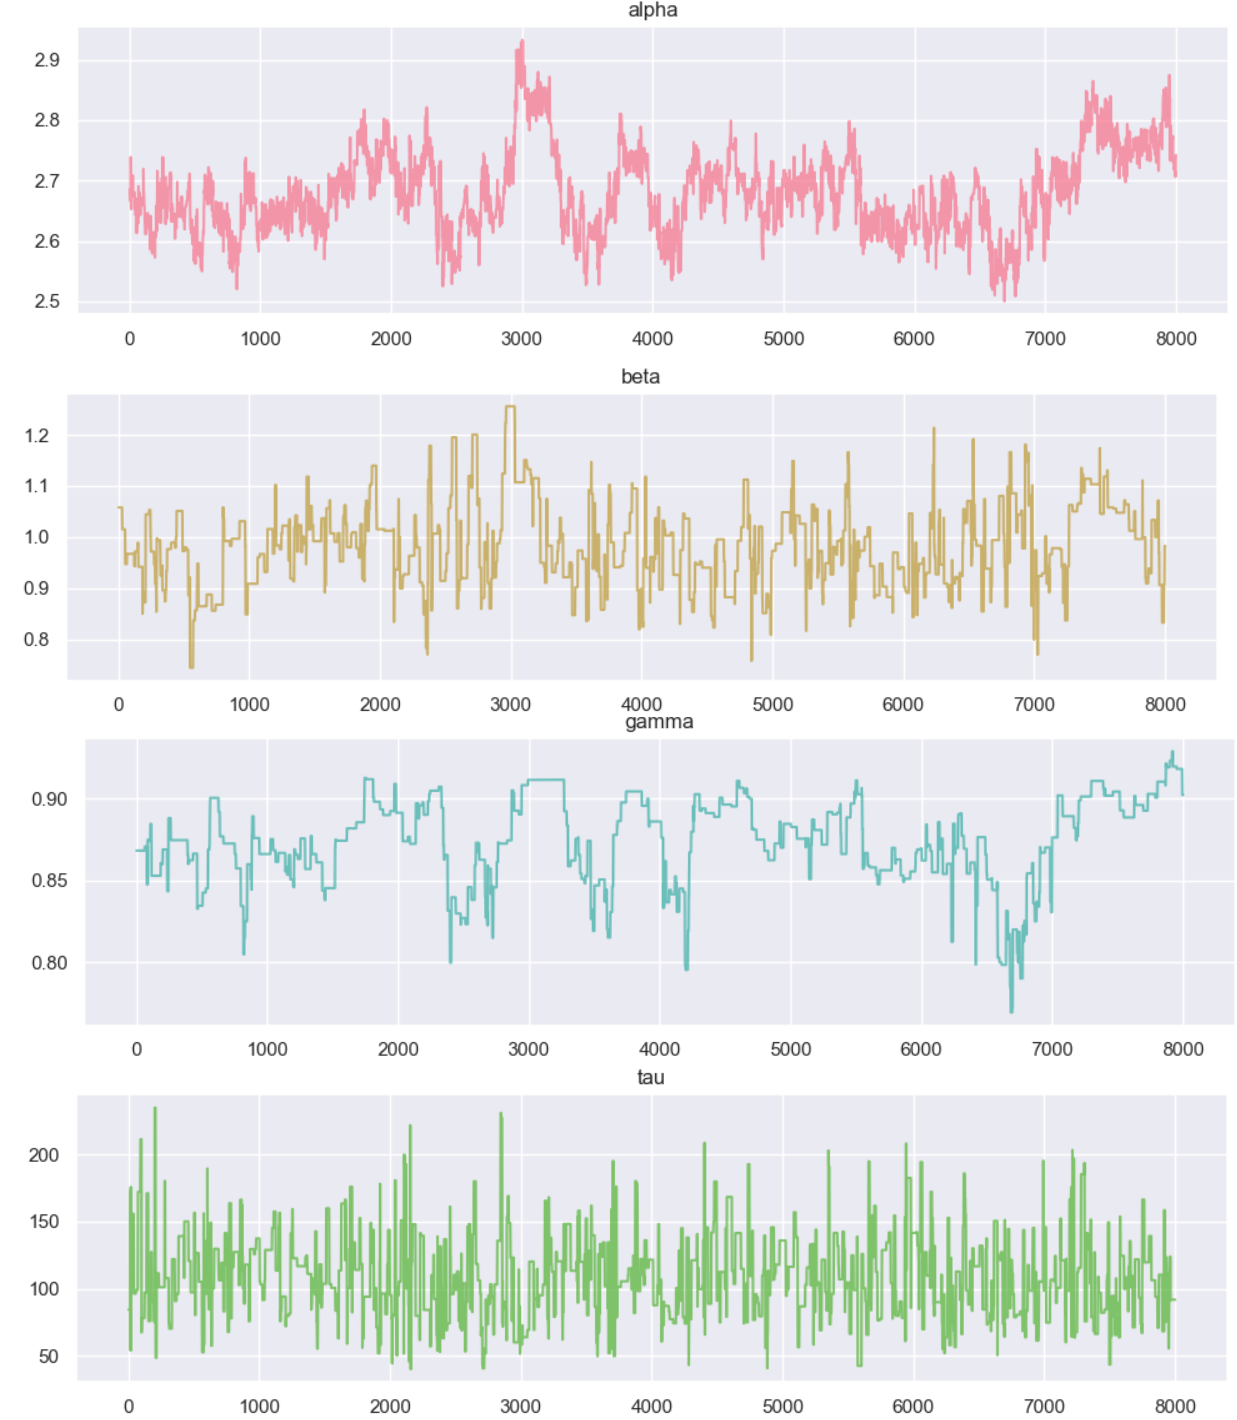
\includegraphics[width=\textwidth]{logos/chaines.png}
    \caption{Chaînes de Markov des paramètres estimés}
    \label{fig:fig1}
  \end{minipage}
  \hfill
  \begin{minipage}[b]{0.45\textwidth}
    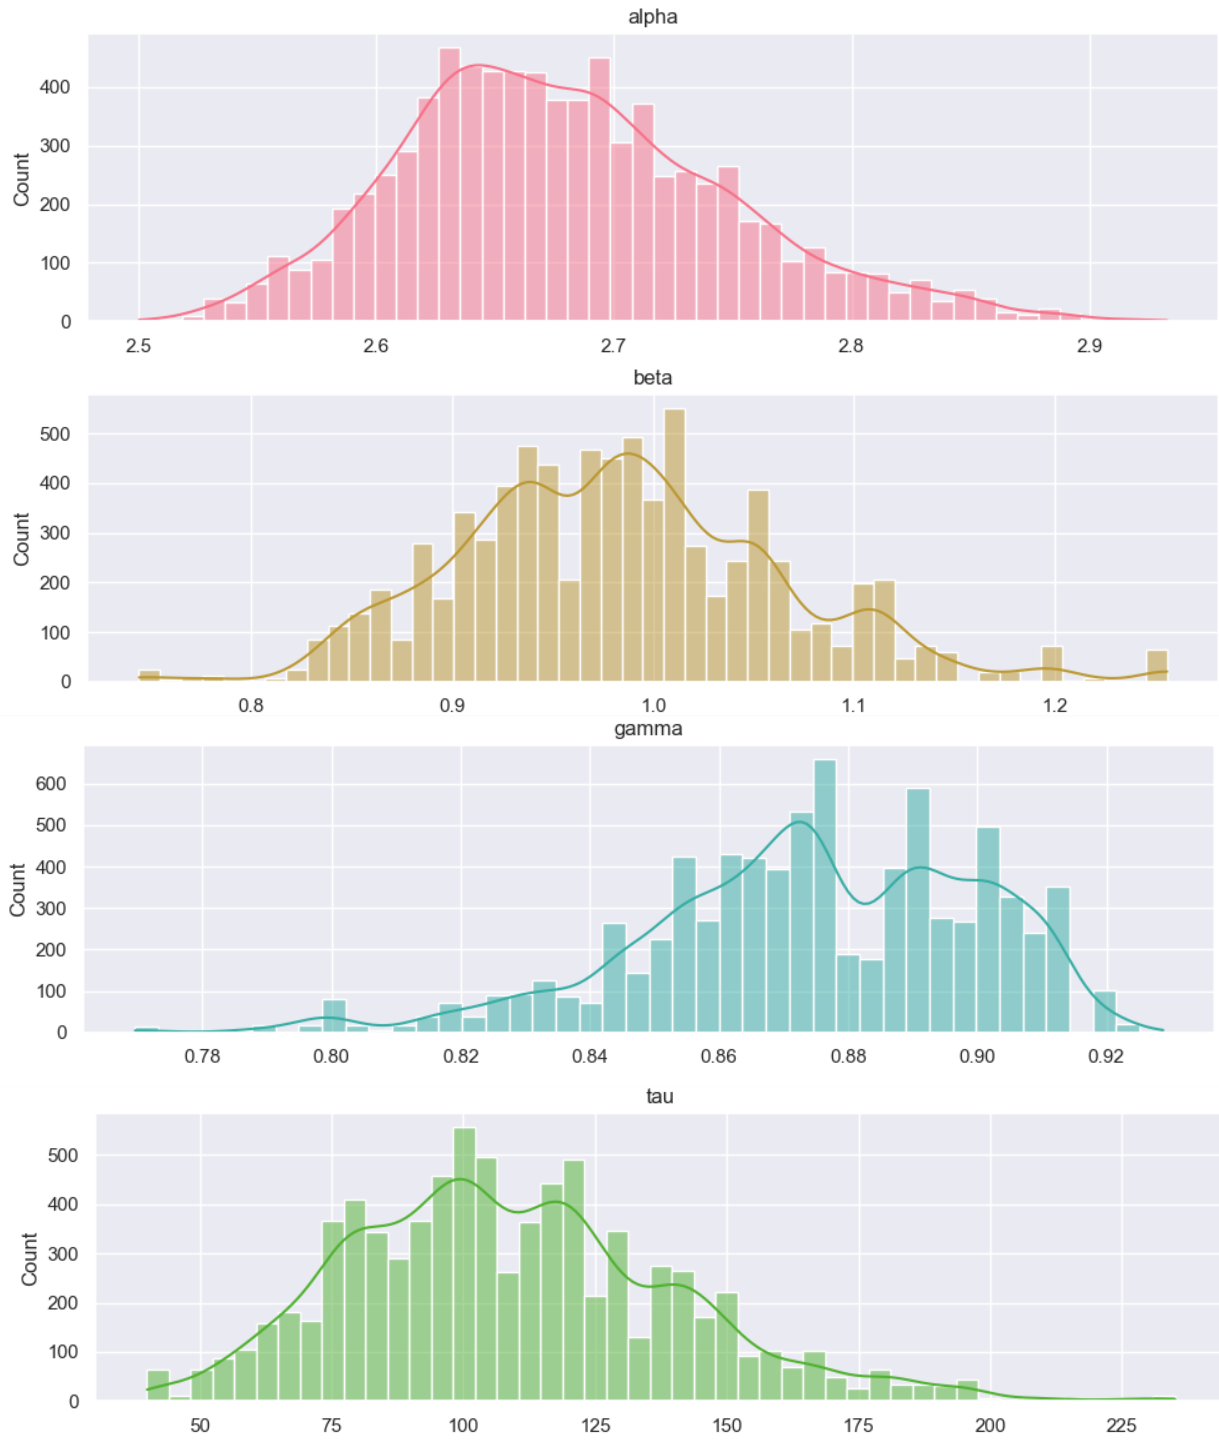
\includegraphics[width=\textwidth]{logos/densites.png}
    \caption{Densité des paramètres estimés}
    \label{fig:fig2}
  \end{minipage}
\end{figure}

Nous pouvons donc comparer les moyennes et les écarts-types des paramètres estimés avec ceux de l'énoncé : 

\begin{table}[h!]
\centering
\begin{tabular}{|>{\centering\arraybackslash}m{1.5cm}|>{\centering\arraybackslash}m{2cm}|>{\centering\arraybackslash}m{2cm}|>{\centering\arraybackslash}m{2cm}|>{\centering\arraybackslash}m{2cm}|}
\cline{2-5}
\multicolumn{1}{c|}{} & \multicolumn{2}{c|}{Moyenne} & \multicolumn{2}{c|}{Écart-type} \\
\cline{2-5}
\multicolumn{1}{c|}{}  & Estimation & Référence & Estimation & Référence \\
\hline
$\alpha$              & 2.651705    & 2.652  & 0.083287    & 0.07094  \\
\hline
$\beta$             & 0.978081    & 0.9729  & 0.077506    & 0.07649  \\
\hline
$\gamma$             & 0.099668    & 0.0992 & 0.014793    & 0.01496  \\
\hline
$\sigma$              & 0.859035  & 0.8623  & 0.040543    &  0.03259 \\
\hline
\end{tabular}
\caption{Résultats et énoncés des paramètres}
\label{table:1}
\end{table}


En mettant en parallèle nos résultats avec les valeurs de référence, on peut voir que nos estimations se rapprochent de ce qu'on attendait. Ça nous montre que notre mise en place de l'algorithme de Gibbs fonctionne bien et que notre modèle est adapté pour analyser les données de cette recherche. \newline

Même si nos estimations se rapprochent des valeurs de référence, il y a toujours une incertitude qui vient avec l'utilisation de l'algorithme de Gibbs pour estimer les paramètres. Cette incertitude se voit dans les intervalles de crédibilité, qui nous donnent une idée de l'éventail où les vrais paramètres pourraient se trouver avec une certaine probabilité.
\begin{figure}[H]
\centering
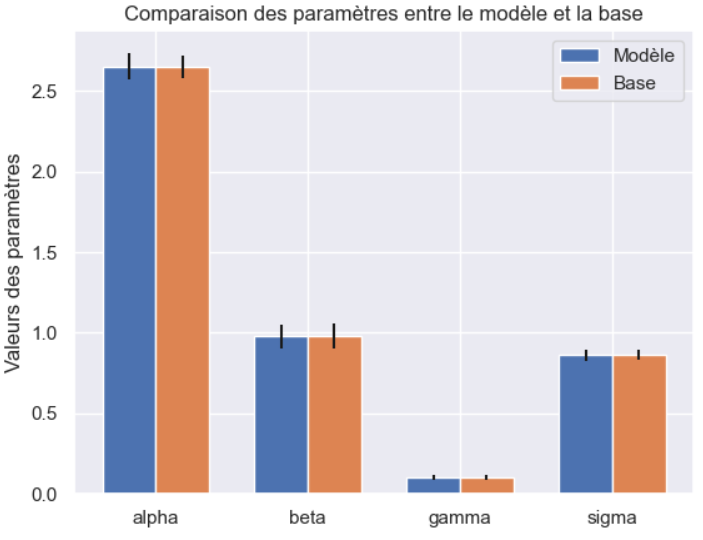
\includegraphics[width=0.6\textwidth]{logos/base.png}
\caption{Comparaison entre les données estimées et les données de référence}
    
\end{figure}


\subsection*{Interprétation}

La valeur obtenue pour $\beta$, approchant 1, indique que notre modèle se rapproche d'un modèle exponentiel modifié. De plus, le fait que $\gamma$ soit près de 0 suggère que la croissance en longueur des dugongs en fonction de leur âge est rapide. Quant à $\alpha$, sa moyenne correspond bien aux données et au problème étudié, car elle est proche de la valeur maximale de Y (2,72). Enfin, la valeur de $\sigma$ démontre que les écarts entre les données et leurs moyennes sont minimes. En exploitant les moyennes de nos chaînes de Markov, nous traçons la progression de la moyenne de $Y_i$ par rapport à l'âge. La courbe confirme que la longueur moyenne des dugongs s'accroît en fonction de l'âge.
\begin{figure}[H]
\centering
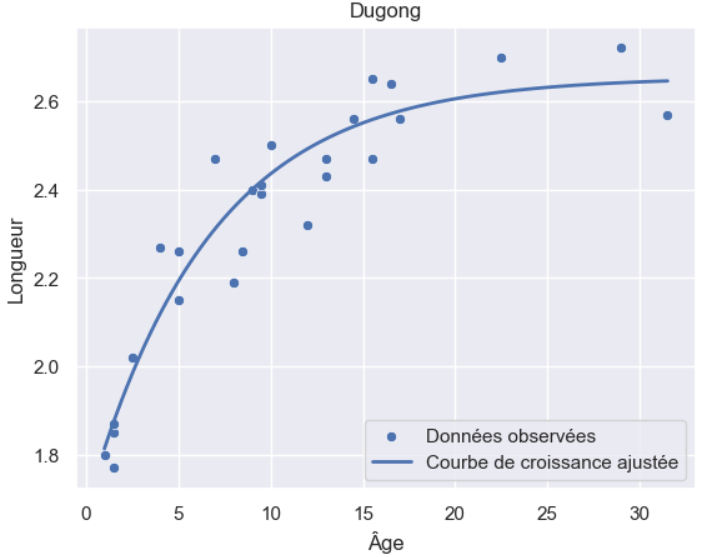
\includegraphics[width=0.4\textwidth]{logos/ev2.png}
\caption{Taille des dugongs en fonction de leur âge}
    
\end{figure}

\end{document}